10. \begin{figure}[ht!]
\center{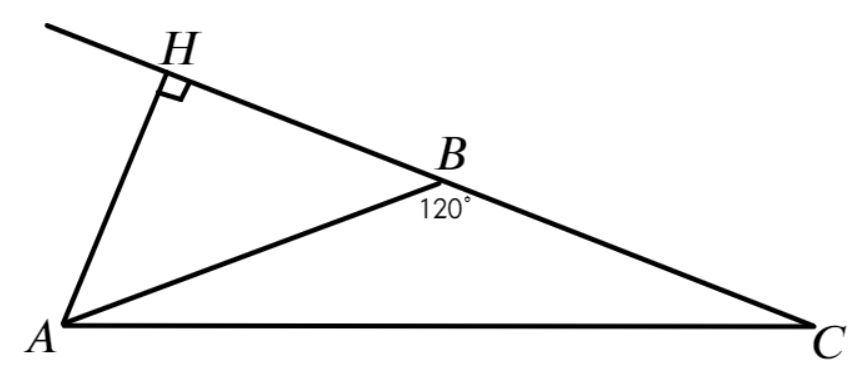
\includegraphics[scale=0.35]{g8-9.png}}
\end{figure}\\
Найдём $\angle C=\cfrac{1}{2}\left(180^\circ-120^\circ\right)=30^\circ.$ Тогда в прямоугольном треугольнике $AHC$ катет $AH$ лежит напротив угла в $30^\circ,$ а значит равен половине гипотенузы $AC,$ поэтому $AH=\cfrac{1}{2}AC=\cfrac{1}{2}\cdot8=4$см.\\
